\documentclass[m,twoside,intern,palatino]{cgBA}


\usepackage{hyperref}						% Verlinkung von Textstellen
\usepackage{fancyhdr}						% eigener Satzspiegel
\usepackage{hypcap} 						% korrekte Verlinkung von Bildern o..
\usepackage[usenames]{color} 				% Einbindung von Farbe
\usepackage{alltt}							% Umschaltung auf typewriter, z.B. fr Quellcode
\usepackage{enumerate}						% Anpassung nummerierter Listen durch optionalen Parameter


\usepackage{mathtools}
\usepackage{empheq}
\usepackage{fancybox}
\usepackage{fancyvrb}


\usepackage{amsfonts}						%
\usepackage{amssymb}						%	Mathe-Zeugs
\usepackage{amsmath}						%

\usepackage{moreverb}						% Erweiterung der verbatim-Umgebung (zum Einbinden von Code)
\usepackage{array}							% Tabellen
\usepackage{url}
\usepackage{tabularx}

%\usepackage[disable]{todonotes}
\usepackage{todonotes}


%-----------------------------------------------------------------------------------------------------------
%own stuff, definitions, haxx, etc. ;)

\setcounter{secnumdepth}{7} %seven levels of nesting
\setcounter{tocdepth}{7}	%
\usepackage{subsections} 	%some definitions for sectionlevelfour up to sectionlevelseven etc ;) need that deep nesting ;(



\graphicspath{{pictures/}}


%stuff to have GLSL syntax highlighing in code listing
\usepackage{listings}
\input{GLSLSyntaxHighlight.tex}

\usepackage{multirow}


%-----------------------------------------------------------------------------------------------------------

\begin{document}

\author{Markus Schl{\"u}ter}
\title{Konzeption und Implementierung eines Unified Rendering Frameworks mit modernen GPU Computing APIs}
\zweitgutachter{Dipl.-Inform.  Dominik Gr{\"u}ntjens}




% Umschalten der Sprache (für englische Rubrikbezeichnungen etc.)
%\selectlanguage{english}


%-----------------------------------------------------------------------------------------------


\maketitle
\clearpage 


\pagenumbering{roman}


\listoftodos		%TODO list, the most important thing in any document ;)
\tableofcontents
\clearpage         	% oder \cleardoublepage bei zweiseitigem Druck
\listoffigures   % fuer ein eventuelles Abbildungsverzeichnis
% \clearpage

\pagenumbering{arabic}


% Hier kommt jetzt der eigentliche Text der Arbeit

\section{Einleitung}
	

Im Rahmen dieser Bachelorarbeit wurde der Frage nachgegangen, inwiefern eine sogenannte "`Unified Rendering-Engine", welche verschiedene Simulationsdomänen vereint, einen Mehrwert darstellen kann gegenüber dem klassischen Ansatz, z.B. gesondert sowohl eine Graphik- als auch eine Physik-Engine zu verwenden, die zunächst einmal keinen
Bezug zueinander haben;\\

Hierbei wurde besonderer Wert auf die Verwendung moderner GPU-Computing-APIs gelegt, namentlich auf OpenGL3/4 und OpenCL.\\
Da bei diesem ganzheitlichen Thema eine vollständige Implementierung einer solchen vereinheitlichten Engine unmöglich war,
konnte nur ein Bruchteil der Konzepte implementiert werden;\\

Dieser Umstand war von Vornherein bekannt, und die Versuchung ist stark, wie in einer Demo die schnelle Realisierung eines Feature-Sets einer konsistenteren, aber zeitaufwändigeren und zunächst karger wirkenden Implementierung vorzuziehen.
Dieser Versuchung wurde versucht, nur dort nachzugeben, wo die negativen Auswirkung auf die Konsistenz des Gesamtsystems lokal bleiben, und so nicht "`Hacks"' sich irreversibel durch das gesamte System ziehen.\\

Letztendlich wurden exemplarisch für die Nutzung in  der visuellen Simulationsdomäne einige gängige visuelle Effekte einer Graphik-Engine implementiert, wie  Shadow Mapping, Normal Mapping, Environment Mapping, Displacement Mapping und dynamisches LOD. Es wurden moderne OpenGL- und Hardware-Features wie Instancing, Uniform Buffers und Hardware-Tesselation verwendet. Schwerpunkt war hier der Einsatz einer Template-Engine, damit
\begin{enumerate}
	\item Boilerplate-Code in den Shadern vermieden wird und
	\item Effekte beliebig (sinnvoll) nach Möglichkeit zur Laufzeit miteinander kombinierbar sind
\end{enumerate}
. Mehr dazu in Kapitel \ref{sec:visualDomain}\\
In der mechanischen Simulationsdomäne wurde eine partikelbasierte Fluidsimulation mit OpenCL auf Basis von Smoothed Particle Hydrodynamics implementiert. Mehr dazu in Kapitel \ref{sec:mechanicalDomain}.\\

Das System trägt den Namen "`Flewnit"', eine bewusst nicht auf den ersten Blick erkennbar sein sollende\footnote{Es soll der generalistische Ansatz des Frameworks nicht in den Hintergrund gedrängt werden.} Kombination der Worte "`Fluid"', in Anspielung auf den urspünglichen Zweck einer Bibliothek zur Fluidsimulation und "`Unit"', in Anspielung auf "`Unity"'-"`Einheit"'. Zufälligerweise ist das $Nit$ auch noch die englische Einheit für die Leuchtdichte, $Cd \over m^2$.


\subsection{Motivation}

Ursprünglich als Arbeit zur Implementierung einer Fluidsimulation geplant, wurde bald ein generalistischer, eher softwaretechnisch orientierter Ansatz verfolgt, der jedoch die Implementierung einer Fluidsimulation mittelfristiges Ziel hatte;\\

\subsubsection{"`Unified Rendering Engine"'}
Der Wunsch nach einer "`Unified Rendering Engine" erwächst aus eigener Erfahrung der Kopplung von Physik- und Graphik-Engines, namentlich der Bullet Physics Library\footnote{http://bulletphysics.org} und der OGRE Graphik-Engine\footnote{http://www.ogre3d.org}. Diese Hochzeit zweier Engines, die jeweils für verschiedene "`Simulationsdomänen"' zuständig sind, bringt gewissen Overhead mit sich, da Konzepten wie  Geometrie und ihrer Transformationen unterschiedliche Repräsentationen bzw. Klassen zugrunde liegen;
Hierdurch wird die gemeinsame Nutzung beider Domänen von Daten wie z.B. Geometrie nahezu unmöglich; Ferner müssen für eine die beiden Engines benutzende Anwendung diese Klassen mit ähnlicher Semantik durch neue Adapterklassen gewrappt werden,
um dem Programmier der eigentlichen Anwendungslogik den ständigen Umgang mit verschiedenen Repräsentationen und deren Synchronisation zu ersparen.\\

\todo{evtl. beispielschema erstellen für zwei klassischee transformationsklassen und adapter vs. unified transformation}

Die Aussage "`Photorealistische Computergraphik ist die Simulation von Licht"' \todo{Zitat einfügen? Stefan Müller, PCG? ;)} hat mich wohl auch inspiriert, den Simulationsbegriff allgemeiner aufzufassen und das Begriffspaar "Rendering und Physiksimulation"' zu hinterfragen\footnote{Auch wenn dieses Framework nicht vornehmlich auf physikalisch basierte, also photorealistische Beleuchtung ausgelegt ist, soll diese aufgrund des generalistischen Konzepts jedoch integrierbar sein.}.

Es sei bemerkt, dass weder eine Hypothese bestätigt noch widerlegt werden sollte, geschweige denn überhaupt eine (mir bekannte) Hypothese im Vorfeld existierte; Es sprechen etliche Argumente für eine Vereinheitlichung der Konzepte (geringerer Overhead durch Wegfall der Adapterklassen, evtl. Speicherverbrauch durch z.T. gemeinsame Nutzbarkeit von Daten), aber auch einige dagegen (Komplexität eines Systems, Anzahl an theoretischen Kombinationsmöglichkeiten steigt, viele sind unsinnig und müssen implizit oder explizit ausgeschlossen werden).\\

Für mich persönlich bringt die Bearbeitung dieser Fragestellung zahlreiche Vorteile; Ich muss ein wenig ausholen:\\
Schon als Kind war ich begeistert von technischen Geräten, auf denen interaktive Computergraphik möglich war; Sie sprechen sowohl das ästhetische Empfinden an, als auch bieten sie eine immer mächtigere Ergänzungs- und  Erweiterungsmöglichkeit zu unserer Realität an; Letztendlich stellten diese Geräte für mich wohl auch immer ein Symbol dafür dar, in wie weit die Menschheit inzwischen fähig ist, den Mikrokosmos zu verstehen und zu nutzen, damit demonstriert, dass sie zumindest die rezeptiven und motorischen Beschränkungen seiner Physiologie überwunden hat.\\
Die Freude an Schönheit und Technologie findet für mich in der Computergraphik und der sie ermöglichenden Hardware eine Verbindungsmöglichkeit; Die informatische Seite mit seinen Algorithmen als auch die technische Seite mit seinen Schaltungen faszinieren mich gleichermaßen; Auch das "`große Ganze" der Realisierung solcher Computergraphischen Systeme, das Engine-Design mit seinen softwaretechnischen Aspekten, interessiert mich.\\
Ferner wollte ich schon immer "die Welt verstehen", sowohl auf physikalisch-naturwissenschaftlich-technischer, als auch - aufgrund der system-immanenten Beschränkungen unseres Universums - auf metaphysischer Ebene\footnote{ob der Begriff "`Verständnis"' im letzten Falle ganz treffend ist, bleibt Ermessens-Sache};\\

Und hier schließt sich der Kreis: Sowohl in der Philosophie als auch in der Informatik spielt das Konzept der Abstraktion eine wichtige Rolle; Nichts anderes tut eine "`Unified Engine": sie abstrahiert bestehende Konzepte teilgebiets-spezifischer Engines, wie z.B. Graphik und Physik; Ich erhoffe mir, dass mit dieser Abstraktion man in seinem konzeptionellen Denken der der realen Welt ein Stück weit näher kommt; Die verfügbaren Rechenressourcen steigen, die Komplexität von Simulationen ebenfalls; Ob eine semantische Generalisierung von seit Jahrzehnten verwendeten Begriffen wie "`Rendering"' und "`Physiksimulation"', welche dieser Entwicklung angemessen sein soll, eher hilfreich oder verwirrend ist, kann eine weitere Interessante Frage sein, die ich jedoch nicht weiter empirisch untersucht habe.\\

Letzendlich verbindet dieses Thema also viele meiner Interessen, welche die gesamte Pipeline eines Virtual-Reality-Systems,  vom Konzept einer Engine bis hin zu den Transistoren einer Graphikkarte, auf sämtlichen Abstraktionsstufen betreffen: Es gab mir die Möglichkeit,
\begin{itemize}
	\item den Mehrwert einer Abstraktion gängiger Konzepte von Computergraphik und Physiksimulation zu erforschen
	\item meine Erfahrung im Engine-Design zu vertiefen
	\item meine Erfahrungen im (graphischen) Echtzeit-Rendering zu vertiefen
	\item mich mit Physiksimulation (genauer: Simulation von Mechanik) zu beschäftigen, konkret mit Fluidsimulation
	
	\item mich in OpenGL 3 und 4 einzuarbeiten, drastisch entschlackten Versionen der Graphik-API, deren gesäuberte Struktur die Graphikprogrammierung wesentlich generalistischer macht und somit die Abstraktion erleichtert
	\item mich in OpenCL einzuarbeiten, den ersten offenen Standard für \linebreak GPGPU\footnote{General Purpose Graphics Processing Unit- Computing, die Nutzung der auf massiver Paralleltät beruhenden Rechenleistung von Graphikkarten in nicht explizit Graphik-relevanten Kontexten}
	\item  mich intensiver mit Graphikkarten-Hardware, der zu Zeit komplexesten und leistungsfähigsten Consumer-Hardware zu beschäftigen, aus purem Interesse und um die OpenCL-Implementierung effizienter zu gestalten

\end{itemize}

\subsubsection{Fluidsimulation}
Warum Fluid?
 interesse an physik, "seichter einstieg" durch verinfachte Algorithmen, so lange es "nur" um plausibilität geht und nicht um physikalische korrektheit, einfacheres Mapping der homogh
Warum Partikelbasiert?
... theoretisch unendliche simulationsdomäne, direkte darstellungsmöglichkeit als openGL vertices, damit directe nutzung von CL/GL interop und somit gemeinsamer nutzung von daten ind beiden domänen..., einfachere mathematik dank lagrange'scher betrachtung, kein advektionsterm, besser einsetzbar für Liquide, da Voxelbasierte ansätze "tricksen" müssen, um das volumen einer teilmenge eines Fluids zu bbewahren;

\clearpage

	
\section{Überblick}
	
\subsection{Vision}

Die langfristige Vision, die \emph{Flewnit} begleitet, ist die Entwicklung eines interaktiven Paddel-Spiels unter Verwendung dieser Unified Engine mit ausgefeilter Fluid-Mechanik und -Visualisierung, partikelbasierten Rigid Bodies und Dreiecks-Mesh als Repräsentation für statische Kollisions-Geometrie; Spiele, in der große Mengen Fluid, die komplexer simuliert sind als durch Height-Fields
\footnote{s. Kapitel \ref{sec:relatedWork} für mehr Informationen zu Height-Field-basierter Fluidsimulation}
einen integrativen Bestandteil der Spielmechanik ausmachen, sind mir nicht bekannt;\\
Von Dreiecks-Geoemetrie erhoffe ich mir eine genauere Repräsentation zur Kollisionsbehandlung, bei gleichzeitiger Ersparnis vieler Partikel, die sonst z.T große Oberflächen repäsentieren müssten; Ferner könnte die Dreiecksstruktur später zur Simulation nicht-partikelbasierter Rigid Bodies verwendet werden;


\subsection{Paradigmen}
\label{sec:paradigm}

Vor dem Entwurf eines komplexen Softwaresystems mit einigen Zügen, die in etablierten Systemen keine so große Bedeutung haben, hat es Sinn, sich einige Paradigmen zu überlegen, welchen das System nach Möglichkeit folgen soll, um eine gewisse Konsitenz zu gewährleisten:
	
\begin{itemize}
	\item Es wurde beim Entwurf der Unified Engine für jede Simulationsdomäne eine möglichst ähnliche Struktur von Klassen 	
	und ihren Beziehungen zueinander angestrebt. Diese Ähnlichkeit spiegelt sich nach Möglichkeit in einer gemeinsamen 	
	(manchmal abstrakten) Oberklasse eines jeden Konzeptes wider, wie z.B.:
	\begin{itemize}
		\item dem Simulations-Objekt als solchem
		\item der Geometrie
		\item dem Material
		\item der Szenen-Repräsentation
	\end{itemize}

	\item Es sollte eine Art Pipeline-Architektur entstehen, wo bestimmte Pipeline-Stages bestimmte Simulations-(Zwischen)-
	Ergebnisse implemetieren, und ggfs. anderen Stages diese zur Verfügung stellen. Jede Simulationsdomäne hat seine eigene 
	Pipeline; Dennoch können Interdependenzen bestehen;\\
	Diesen Interdependenzen wird durch eine Konzept-spezifische Verwaltung durch verschiedene Singleton-Manager-Klassen 	
	genüge getan; Ein und dasselbe Objekt kann von verschiedenen Managern in unterschiedlichem Zusammenhang verwaltet 
	werden; Mehr dazu in Kapitel \ref{sec:systemArchitecture};

	\item Es sollen langfristig so viele Features (Visualisierungstechniken und -effekte, Simulationstechniken) wie möglich 
	miteinander kombinierbar sein, sofern die Kombination nicht unsinnig ist;

	\item Es soll so viel wie möglich auf der GPU berechnet werden, um die massive Paralleltät auszunutzen, 
	und um nicht durch Buffer-Transfers, die die Aufteilung von Algorithmen in CPU- und GPU- Code meist mit sich bringen, 	
	auf den Bandbreiten- und Latenz- Flaschenhals der PCI-Express-Schnittstelle zu stoßen;
	\todo{hier specs und refs zu PCIe 2.0 anbringen? eher nicht, oder?}
	
	\item Es soll immer das Potential gewahrt werden, dass aus dem Framework --- außerhalb des Rahmens dieser 
	Bachelorarbeit --- tatsächlich noch eine Art \emph{Unified Engine} entstehen kann; Somit sind "`schnelle Hacks"',
	also unsaubere Programmier-Weisen, die mit geringstem Programmier-Aufwand ein bestimmtes Feature implementieren,
	überall dort unbedingt zu vermeiden, wo sie die konsistente Gesamstruktur des Systems zu bedrohen scheinen.

\end{itemize}



	


\subsection{Begriffe}

Im Zuge der angestrebten Vereinheitlichung der  verschiedenen Simulation müssen wir auch einige Begriffe verallgemeinern, 
welche in ihrer jahrzentelangen Tradition in der Terminologie der Computergraphik eine spezifische Bedeutung erhalten haben;
Zur besserern Einordnung stellt Abbildung \ref{fig:classicalVsUnified} ein grobes Schema dar, welches die klassische Verwendung verschiedener Engines und die einer Unified Engine gegenüber stellt:



	\begin{figure}
		%\centering
	
	   %\def\svgwidth{1.6\textwidth}
	   %\input{classicalVsUnified.pdf_tex}
		%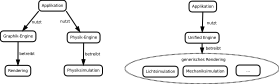
\includegraphics[width=1.3\textwidth]{classicalVsUnified.png}
	   %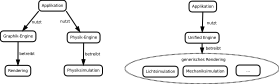
\includegraphics[width=1.3\textwidth]{classicalVsUnified.pdf}
	   \includegraphics[width=1.3\textwidth]{screenshot_wholeScene.png}

		\caption{Gegenüberstellung von Verwendung und Begrifflichkeiten von klassischen Engines und einer Unified Engine}
		\label{fig:classicalVsUnified}
	\end{figure}
	




\begin{description}

	\item[Rendering]
	Im Wiktionary \cite{internet:wiktionRender} wird das Verb \emph{to render} u.a. umschrieben als:
	\begin{quote}
		(transitive, computer graphics) To transform digital information in the form received from a repository into a 
		display on a computer screen, or for other presentation to the user. 
	\end{quote}	
	Es geht also um die Transformation einer formalen Beschreibung in eine für einen menschlichen Benutzer wahrnehmbare 
	Form. Diese muss entgegen der gewöhnlichen Verwendung des Begriffes nicht zwingend visuell, sondern kann z.B. auch 
	akustischer oder haptischer Natur sein, übertragen durch Lautsprecher oder Force-Feedback-Devices.\\
	
	Verallgemeinern wir den Begriff \emph{Rendering} weiter, gemäß der Übersetzung der Verb-Form als 
	\emph{erbringen}, \emph{machen} \cite{internet:dictCCrender},	
	und in Anlehnung an seine Ethymologie,
	\begin{quote}
		From Old French \emph{rendre} (“to render, to make”) [...] \cite{internet:wiktionRender}
	\end{quote}
	
	bietet sich eine freie Übersetzung als \emph{Erzeugung eines Zustandes beliebiger Natur} an;\\
	Unter diese generische (Um)-Deutung des Begriffes fällt nun auch \emph{die Ausführung beliebig gearteter Simulation}.
	
	Zu besseren Abgrenzung kann man von \emph{generischen Rendering} und dem klassischen 
	\emph{visuellen Rendering} sprechen; Dies soll im weiteren Verlauf dieser Arbeit der Fall sein.\\
	Eine \emph{Unified Engine}(s.u.) betreibt also \emph{generisches Rendering}.
	
	
	\item[Unified Engine] Alternativ-Bezeichnung: \emph{Unified Rendering Engine};\\
	Eine \emph{Unified Engine} betreibt \emph{generisches Rendering}, indem sie bestimmte Aspekte einer 
	\emph{Welt}\footnote{Diese Welt muss dabei nicht zwingend unserer Realität ähneln oder entsprechen.} simuliert. 
	Darunter kann das klassische (visuelle) Rendering fallen, aber auch die Simulation von Geräuschen und von Mechanik, und 
	beliebige weitere Domänen; Die Domänen sollen dabei durch Abstraktion gemeinsamer Eigenschaften so ähnlich wie möglich
	organisiert sein;
	
	\item[Simulation] Das Begriffspaar \emph{Rendering} und \emph{Physiksimulation} ist im Kontext dieser versuchten 
	Vereinheitlichung nicht mehr angemessen; 
	

	
	%don't know yet if it makes sense here to define the below words
	%\item[Material] 
	%\item[Buffer] 

	
\end{description}

erklären, was ich unter Unified Rendering verstehe, was Rendering dadruch fuer eine generalistische Bedeutung bekommt;\\
tabelle mit Gegenüberstellung




\subsection{Schwerpunkte}

	- entwicklungsumgebungm die die entwicklöung eines konsistenten frameworks erleichtert, moderne tools, nach möglichkeit cross platform (windows vs. linux)
	- verwendung von bibliotheken, die die entwicklung einer seriösen engine ermöglichen
	- verwendung von mindestens OpenGL 3/3 core context, um legacy code schon zur compilezeit auszuschließen
	- realisierung gängiger graphischer effekte, vor allem tesselation, verweise auf entsprechende section
		- tesselation
	- nutzung moderner openGL features, Uniform Buffers, Tesselation, hardware instancing, verweis auf entpsrechende section;
	- möglichst hohe konfiguriertbarkeit ohne ständigen recompile: config file
	- buffer abstraktion
	- memory tracking, (erklären, warum nicht tracking mit Valgrind)

	- effiziente Verwendung von OpenCL, hardware- spezifische bedingte compilings dank grantlee
	
	

	\subsubsection{Template-Engine}
	boilerplate, kombinierbarkeit, nach Möglichkeit lesbarkeit\\
	exemplarischer code schnipsel
		-  Im Zuge des Schwerpunktes auf GPU-Implementierung:
		grantlee gegen boilerplate,zur generierung schlankerer programme als durch Präprozessordierktiven, 
		 $\rightarrow$ einfachere Code- Inspection, verbesserung der lesbarkeit durch generierte, feature-spezifische 	
		 programme,
  		bessere struktur verwaltung des source codees

	\subsubsection{Performance duch Implementierung auf der GPU mit modernen GPU-Computing-APIs}
	auf die massive parallelität eingehen, die sowohl von visualler wie mechanischer domäne genutzt werden kann;
	Performance-Schwerpunkt, Optimierung, auch hardware-abhängige, erwähnen, Gegenüberstellung zu alten OpenGL-nutzenden 	
	GPUPU- Verfahren, die nicht scattern konnten in texturen rendern mussten und auch sonst etliche Nachteile hinnehmen 	
	mussten

	\subsubsection{Potential der Entwicklung hin zu einer Unified Engine nicht verschenken}
	i.e. fenstermanager, input etc sollten wohl übelegt sein, für vielseitig, flexible anwendung zur Laufzeit sollten keine 	Speicher-Lecks auftreten, damit Funktionalität kontrolliert heruntergefahren und neu initialisiert werden kann; Für 	
	gemeinsamen zugriff sollten viele Daten für andere Klassen verfügbar sein (Buffer, Rendering Results...); Realisierung 	
	uber Manager-Singleton-Klassen und Zugriff über Map-Container;


	


\section{Systemarchitektur}
	
\label{sec:systemArchitecture}

Dieses Kapitel soll ein Gefühl für die Komponenten von \emph{Flewnit} und 
ihre Zusammenhänge vermitteln. Die Komponenten "`in Aktion"' werden im Detail im Verlauf des Kapitels 
\ref{sec:simulation} beschrieben.

Das System wurde in C++ als (wahlweise statisch oder dynamisch zu linkende) Bibliothek implementiert.
Der Code der GPU-Programme ist in GLSL bzw. OpenCL C verfasst.

\subsection{Dependencies}
	\label{sec:dependencies}
	
	Zunächst sollen die verwendeten Third-Party-Bibliotheken kurz vorgestellt werden:

	\begin{description}
		\item[OpenGL3/4]
		Die schon mehrfach erwähnten modernen Versionen der \linebreak \emph{Open Graphics Library},
		der offenen API der Khronos Group zur \linebreak hardwarebeschleunigten Graphik-Programmierung 
		auf Basis der Dreiecks-Rasterisierung.
		\todo[color=green]{evtl treffenderen Ausdruck finden: Scanline-basiert oder was auch immer}
		Um die Programmierung ohne Legacy-Routinen nicht erst zur Laufzeit über einen OpenCL-Error
		durch Verwendung eines Core-Profiles zu erzwingen, gibt es einen OpenGL- Header
		namens "`gl3.h"'\footnote{beziehbar unter http://www.opengl.org/registry/},
		der in Kombination mit der entsprechenden Präprozessor-Definition
		\lstinline[language=C]|#define GL3_PROTOTYPES 1| schon zur Compile-Zeit nur die non-deprecated
		Routinen zur Verfügung stellt.
		
     	\item[OpenCL 1.0]
	    Die \emph{Open Computing Language}, erste Version der noch jungen API für massiv parallele Programmierung
	    \footnote{die GPGPU-Computing einschließt}, wie OpenGL von der Khronos Group verwaltet; 
	    sie stellt den ersten offenen Standard für GPGPU dar, d.h., die Verwendung der API ist nicht mehr an eine
	    bestimmte Hardware (wie bei Nvidia CUDA) oder ein bestimmtes Betriebssystem (wie Microsofts DirectCompute)
	    gebunden.
	    
	    Zur Zeit der Implementierung waren noch keine Non-Developer-Treiber für OpenCL 1.1 verfügbar, 
	    außerdem gab es kein Feature dieser Version, welches ich dringend benötigt hätte.
	    Deshalb habe ich die Version 1.0 verwendet.
	    
	    Es gibt einen C++ -Wrapper der C-API, welcher stark auf C++-Templates basiert und in einer einzigen Headerdatei 
	    implementiert ist. Dieser ist direkt von der Khronos-Homepage\footnote{http://www.khronos.org/registry/cl/} 	
	    beziehbar. Diesen Wrapper habe ich verwendet, da er die Nutzung der API wesentlich eleganter macht.
	    
    	
   		\item[GLFW 2.7]
		Wie auf Seite \pageref{focus:dependencies} angedeutet, waren mir folgende Dinge wichtig, damit die Einsetzbarkeit
		des Frameworks in professionelleren Kontexten nicht schon im Vorfeld verbaut ist:
		\begin{itemize}
			\item Option auf Fullscreen
			\item Option auf Multisampling
			\item Die Möglichkeit der Erstellung eines OpenGL-Kontextes einer frei wählbaren Version 
			mit Option zwischen Core- und Compatibility-Profile
			\item Option auf "`\emph{Mouse Grab}"', so dass man wie in einem Computerspiel mit ausgeblendetem Mauszeiger
			nur durch Bewegung der Maus ohne Bildschirm-/Fenster-Grenzen die virtuelle Kamera rotieren kann;
			\item "`Input events"', d.h. Aktualisierungen von Benutzereingaben sollen häufig und mit minimaler 
			Latenz geschehen, außerdem so unabhängig wie möglich von der Framerate sein;
			Nach möglichkeit sollten Input-Updates zumindest "aktiv abfragbar" sein 
			(im Gegensatz zum passiven Warten darauf, dass von der Input-Library eine Callback-Funktion 
			aufgerufen wird)
			\item Es soll volle Kontrolle über die "Render-Loop" geben, so dass man nicht 
			den Kontrollfluss an eine Funktion übergibt, die womöglich nie zurückkehrt und weiteren Kontrollfluss
			durch das Benutzerprogramm	nur über Callback-Funktionen ermöglicht
			(wie \lstinline[language=C]|glutEnterMainLoop()| beim in die Jahre gekommenen \emph{GLUT}).
			Ein derartiges Konstrukt ist einer
			Engine nicht würdig und verhindert womöglich sauberes Herunterfahren und Neu-Initialisierung,
			wie es z.B. beim Wechseln einer Szene oder eines fundamentalen globalen Settings nötig sein könnte.	
		\end{itemize}
		\emph{GLFW}\footnote{http://www.glfw.org/} in der Version 2.7, die zum Zeitpunkt der Implementation aktuellste 
		stabile	Version, erfüllt diese Forderungen, und findet damit in \emph{Flewnit} Einsatz sowohl im Fenster- als auch 	
		im Input-Manager. Die Timing-Funktionalität wird ebenfalls von GLFW übernommen.
		
    	
    	\item[GLM]
    	leichte, aber doch recht maechtige mathe-bibliothek
    	
    	\item[Grantlee]
       		die string template engine die CL und GL code erzeugt
       		
    	\item[assimp]
    	

		\item[boost filesystem]
    	
   		\item[TinyXML]
    	- möglichst hohe Konfiguriertbarkeit ohne ständigen recompile: parsing von XML config file
	
	\end{description}	

	
	

    

    	
 

\subsection{Klassendiagramm}

\begin{figure}[!h]
	 \includegraphics[width=\textwidth]{Overview_Flewnit_Architecture_After_Implementation1.pdf}
	\caption{Klassendiagramm des Gesamtsystems, Teil 1}
	\label{fig:ClassDiagOverview1}
\end{figure}


\begin{figure}[!h]
	 \includegraphics[width=\textwidth]{Overview_Flewnit_Architecture_After_Implementation2.pdf}
	\caption{Klassendiagramm des Gesamtsystems, Teil 2}
	\label{fig:ClassDiagOverview1}
\end{figure}



 
\subsection{BasicObject und Memory Tracking}
	 für vielseitig, flexible anwendung zur Laufzeit sollten keine 	Speicher-Lecks auftreten damit Funktionalität 
	 kontrolliert heruntergefahren und neu initialisiert werden kann; 
	 	- memory tracking, (erklären, warum nicht tracking mit Valgrind)
 
    	
\subsection{Die \emph{Unified Rendering Engine}}
URE blubb

\subsection{Die Simulator-Klassen}


\subsection{Die SimulationPipelineStages}
	shdow map gen, direct lighting, rendering features particlemechanics stage;
	in planung: deferred rendering G-Bufferfill, deferred rendering shade, div. post processing stages


\subsection{Die Manager-Klassen}
Für gemeinsamen zugriff sollten viele Daten für andere Klassen verfügbar sein (Buffer, Rendering Results...); 	
Realisierung über Manager-Singleton-Klassen und Zugriff über Map-Container;
\todo[color=green]{evtl. andere reihenfolge}

\subsection{Die Template-Engine}
	\label{sec:architecture:templateEngine}
	exemplarischer code schnipsel, refernz su shadermanager und CLProgramManager, erklärung wie man templat contex setzt, 	
	vererbung etc;
    	
\subsection{Die Buffer-Abstraktion}  
	\label{sec:architecture:BufferAbstraction} 	
 	die bombe, die cpu, ogl und ocl vereint, inclusive ping ponging etc.. 
 	fundamentale Klassensammlung fuer den Unified-Aspekt
 	
 	\begin{figure}[!h]
  		\begin{tabular}
  		{
  		 l  l | c | c | c |
  		}
																	\cline{3-5}
  									&								&	\multicolumn{3}{ c | }{Context} \\ 
  																	\cline{3-5}
									&								& 	Host 	& 	OpenGL 	& 	OpenCL	\\
    	\noalign{\hrule}								
    	\multicolumn{1}{|c|}{
    		generic Buffer
    	}							& 								
    		&	{\color{green}\checkmark} 	&	{\color{red}x}		& 	{\color{green}\checkmark}	\\ 
    	
    	\noalign{\hrule}								
    	\multicolumn{1}{|c|}{
    		\multirow{4}{*}{OpenGL Buffers}
    	}							& Vertex Attribute Buffer		
    		&	{\color{orange}o} 	&	{\color{green}\checkmark}		& 	{\color{orange}o}	\\  
    								\cline{3-5}
    	\multicolumn{1}{|c|}{}		& Vertex Index Buffer			
    		&	{\color{orange}o} 	&	{\color{green}\checkmark}		& 	{\color{orange}o}	\\  
    								\cline{3-5}
    	\multicolumn{1}{|c|}{}		& Uniform Buffer
    		&	{\color{orange}o} 	&	{\color{green}\checkmark}		& 	{\color{orange}o}	\\ 
    								\cline{3-5} 
    	\multicolumn{1}{|c|}{}		& Render Buffer					
    		&	{\color{red}x} 	&	{\color{green}\checkmark}		& 	{\color{green}\checkmark}	\\ 
    
   		\noalign{\hrule}								
   		\multicolumn{1}{|c|}{
    		\multirow{4}{*}{Textures} 
   		}							& 1D Texture					
   			&	{\color{orange}o} 	&	{\color{green}\checkmark}		& 	{\color{red}x}	\\ 
    								\cline{3-5}
		\multicolumn{1}{|c|}{}		& 2D Texture				
			&	{\color{orange}o} 	&	{\color{green}\checkmark}		& 	{\color{green}\checkmark}	\\ 
									\cline{3-5}
		\multicolumn{1}{|c|}{}		& 3D Texture		
			&	{\color{orange}o} 	&	{\color{green}\checkmark}		& 	{\color{green}\checkmark}	\\ 
									\cline{3-5}
		\multicolumn{1}{|c|}{}		& Special Texture				
			&	{\color{orange}?} 	&	{\color{green}\checkmark}		& 	{\color{orange}?}	\\ 


    	\noalign{\hrule}
     
     	
  		\end{tabular}	
  	
  		\caption{		
  			Verschiedene Buffertypen und ihre Verfügbarkeit in verschiedenen Kontexten \\	
  			Legende: \\
			{\color{green}\checkmark}	$\rightarrow$ nativ unterstützt;
			{\color{orange}o}	$\rightarrow$ kompatibel;
			{\color{red}x}	$\rightarrow$ nicht unterstützt;	\\
			{\color{orange}?}	$\rightarrow$ Unterstützung abhängig von weiteren Parametern;	
		}
	
  	\end{figure}
 
\subsection{Das WorldObject}
	Basis-Klasse fuer alles was unified simuliert wird: pure viuelle objekt, uniform grid, fluid, rigid body etc..
	
	\subsubsection{Das SubObject}
  
 
\subsection{Material}  
	was stellt welches material in welcher Domain dar?
	
\subsection{Geometry}
	Abtract, Buffer based, Vertex based etc.. ein paar konzepte (implementiert/genutzt nur VertexBased)  
	
\subsection{Massively Parallel Program}
	Basisklasse von Shader und OpenCL Program
	\subsubsection{Shader}
		
	\subsubsection{OpenCLProgram}

weitere klassen/konzepte to go...	


\subsection{Status der Implementierung am Ende der BA}
	
	Features auflisten;
	\todo[color=green]{screenshots? oder lieber erst später,zusammen mit detaillierter erläuterung?}

	großteils programmierte, aber ungenutzte/ungetestete features erwähnen (Deferred Rendering, Layered Rendering, 	
	RenderTarget-Klasse, Partikel-Rigid bodies, verschiedene Fluid-Typen); 


	überlegte aber nciht programmierte Konzepte/Algorithmen erwähnen (Triangle-Index-Voxelisierung)
	
	schlimmste schnitzer nennen, wie
		- miese fluid-visualisierung, 
		- unübersichtliche shadertemplates, besser gemacht bei CL-
			Kernel-Templates, 1. weil struktur hier besser "vererbbar", 2. weil mehr erfahrung mit  Template-Engine
	
	  	
  	

\clearpage

	
\section{Simulation}
	\label{sec:simulation}
	\subsection{Die visuelle Simulationsdomäne}
		
	Ein paar worte ueber die shading features, wie sie maskiert werden

\subsection{Der LightingSimulator}
	Nochmal drauf hinweisen, dass Rendering etwas generisches in diesem Framework ist, und wir leiber von Lichtsimulation sprechen sollten, auch wenn es monetan nicht photrealistisch ist ;)
	

\subsection{ShaderManager}
	generiert mit grantlee, assigned an materials und verwaltet Shader , abhaenging von der aktuellen lighting stage, den registierten Materials,
	der Erzeugten kontext, den vom user aktivierten rendering features etc pp
	
\subsection{Instancing}
	InstanManager, InstangedGeometry vorstellen, konzept, wie es verwaltet wird, erklaeren
\subsection{Uniform Buffers}
	auch von BufferInterface abstrahiert, vorteile auflisten, aber auch stolperfallen 8alignment etc)
\subsection{Tesselation}
	basics des hardware features erwaehnen fuer den geneigten leser, raptor-modell erwaehnen und seinen Aufbereitungsprozess, LOD, displacement mapping erlaeutern
	
	  

\clearpage	
	\subsection{Die mechanische Simulationsdomäne}
		

\label{sec:mechanicalDomain}
In dieser Domäne wurde exemplarisch eine partikelbasierte Fluid-Simulation nach dem
Verfahren der Smoothed Particle Hydrodynamics mit OpenCL implementiert.
	
\subsubsection{Fluid-Simulation}
		
	\paragraph{Grundlagen}	
		\subparagraph{Die Navier-Stokes-Gleichungen}
		Die Sammlung an Gleichungen, die das Verhalten von Fluiden beschreiben, sind die
		\emph{Navier-Stokes-Gleichungen}.
		Für die Echtzeit-Simulation nützlich sind die \emph{inkompressiblen} Navier-Stokes-Gleichungen:
		\begin{subequations}\label{equ:navStokes1}
			\begin{align}
			\rho 
			\left( 
				\frac{\partial \vec{v}}{\partial t} 
				+ 
				\left( \vec{v} \cdot \nabla	\right) \vec{v} 
			\right)
				& = - \nabla p  + \mu \Delta \vec{v} + \vec{f} \\
			\nabla \cdot \vec{v}   & = 0
			\end{align}	
		\end{subequations}
		
		Die erste Gleichung heißt \emph{Impulsgleichung}. Die basiert auf dem zweiten Newtonschen Gesetz
		\begin{equation}
			\vec{F} = m \cdot \vec{a}
		\end{equation}
		
		$\rho$ steht für die Dichte  $\frac{m}{V}$, $\vec{v}$ für die Geschwindigkeit, $t$ für die Zeit,
		$p$ für den Druck, $\mu$ ist die Viskosität und $\vec{f}$ steht für sämtliche weiteren
		Kräfte, u.a. Gravitation.\\
		$\nabla$ ist der Nabla-Operator, der den Gradienten einer Größe liefert, 
		$\nabla \cdot$	ist die Divergenz,	
		$\Delta$ ist der Laplace-Operator und ein Maß für die Abweichung einer Größe vom Durchschnitt.\\	
		
		Bei den beschriebenen physikalischen Größen handelt es sich um \emph{Kraft pro Volumen},
		"`Kraftdichten"' (engl. \emph{force density}).
		
		Die zweite Gleichung ist die Inkompressibilitätsbedingung.
		Die Forderung, dass die Divergenz der Geschwindigkeit überall null sein muss, heißt anschaulich, dass es keine
		Quellen oder Senken von Geschwindigkeitsvektoren geben darf. Damit bleibt die Dichte konstant, da immer genauso
		viel Materie einen Punkt verlässt wie "`herein kommt"'.\\

		Der Term 			
		$
				\frac{\partial \vec{v}}{\partial t} 
				+ 
				\left( \vec{v} \cdot \nabla	\right) \vec{v} 
		$
		beschreibt die \emph{Materielle Ableitung} und vereinfacht sich aufgrund der "`Lagrange'schen Natur"'
		der Partikeldomäne zu $\frac{D \vec{v}}{D t}$, da wir keinen Advektions-Term benötigen.\\

		
			
		Eine recht gute Einführung für den Laien in diese nicht ganz intuitiven Formeln, mit ein paar Beispielen
		und Herleitungen, liefert \cite{Steil2007}. Insbesondere wird hier die  
		"`Lagrange'sche"' und "`Eulersche"' Sicht, die über die Materielle Ableitung verknüpft sind,
		an einem anschaulichen Beispiel erläutert.\\
		
		Was wir für den weiteren Verlauf dieses Kapitels aus den Gleichungen \ref{equ:navStokes1} mitnehmen müssen,
		ist, dass wir für die mechanische Simulation von Fluiden Kraftdichten berechnen wollen,
		aus denen wir durch Division durch die Dichte die Beschleunigungen errechnen können,
		mithilfe derer dann die Integration geschieht, also die Aktualisierung von Positionen und Geschwindigkeiten.
			
		
			
				
		\subparagraph{Smoothed Particle Hydrodynamics}
		Das Verfahren wurde eigentlich von \cite{Gingold_Monaghan_1977} für Anwendung in der Astrophysik
		entwickelt, jedoch ist es auch für beliebige Fluidsimulationen einsetzbar.
		Es handelt sich um eine Interpolations-Methode: physikalische Größen sind nur stichprobenhaft
		in einem Raum enthalten, doch durch Interpolation von Nachbar-Samples lässt sich eine Größe $A$
		für jeden Punkt $\vec{r}$ im Raum bestimmen:
		
		\begin{equation} \label{equ:SPHbase}
			A_S(\vec{r}) = \sum_j m_j \frac{A_j}{\rho_j} W(\vec{r}-\vec{r}_j,h)
		\end{equation}
		
		Es wird über die $j$ Nachbar-Partikel in der Umgebung iteriert, und die Quantitäten aufsummiert,
		wobei sie mit dem Volumen ($\frac{m_i}{\rho_i}=V_i$) 
		sowie einem "`radial symmetric smoothing kernel"'  $W(\vec{r}_j,h)$ gewichtet werden.
		$h$ ist hier der \emph{Support Radius}. Der Kernel heißt "`normalisiert"' wenn sein Integral 1 ergibt:
		$\int W(\vec{r}) d \vec{r}=1$.\\
		
		
		Eine wichtige Eigenschaft ist, dass der Gradient oder der Laplacian
		einer Größe wie in Gleichung \ref{equ:SPHbase} zu berechnen ist, nur dass man den Gradienten bzw. den Laplacian
		des Smoothing Kernels verwendet:
		\begin{subequations}\label{equ:navStokes1}
			\begin{align}
			\nabla A_S(\vec{r}) &= \sum_j m_j \frac{A_j}{\rho_j} \nabla W(\vec{r}-\vec{r}_j,h) \\
			\Delta A_S(\vec{r}) &= \sum_j m_j \frac{A_j}{\rho_j} \Delta W(\vec{r}-\vec{r}_j,h)
			\end{align}	
		\end{subequations}
		
		Die Dichte an einem Punkt kann ebenfalls mit Gleichung \ref{equ:SPHbase} berechnet werden, wobei sich 
		gerade diese heraus kürzt:
		
		\begin{equation} \label{equ:SPHbase}
			\rho (\vec{r}) = \sum_j m_j  W(\vec{r}-\vec{r}_j,h)
		\end{equation}
		
		Je nach physikalischer Größe bieten sich unterschiedliche Sommting Kernels an, die besondere
		Eigenschaften haben.		
		
		%Es sei noch ein Wort über die Dichte verloren: Obwohl wir eigentlich inkompressible Flüssigkeiten
		%simulieren wollen, sorgen verschiedene Umstände dafür, dass die Dichte dennoch variiert: numerische Ungenauigkeit,
		%Dämpfung für numerische Stabilitä


		
		%ursprünglich aus astronomie blubb blubb 
		%\todo{überlegen, ob ich aus Interesse nicht noch weiter in die Richtung recherchieren sollte, da ich nach meiner 
		%Implementierung erst so richtig beeindruckt von dem Verfahren war (ich habe im Internet noch keine Fluid-Demo 
		%gefunden, die ebenfalls SPH implementiert; ok., ich hab auch nicht gesucht ;) ), und gerne mehr über die 
		%Hintergründe verstehen würde... problem, wie immer: Zeitdruck ;( }		
		
	\paragraph{Verwandte Arbeiten}
	\label{sec:relatedWork}

	Jos Stam \cite{Stam99stablefluids,Stam03realtimefluid} hat auf dem Gebiet der interaktiven Fluid-Simulation 
	Poinier-Arbeit geleistet 
	
	Referenzen auf Müller03, Thomas Steil, Goswami, GPU gems, Aufzeigen, was ich von wem übernommen habe, was ich selbst  
	modifiziert habe aufgrund von etwaigen Fehlern in den Papers odel weil OpenCL es schlciht nicht zulässt;
	

	\paragraph{Algorithmen}
	Verwaltung der Beschleunigungsstruktur ist der Löwenanteil, nicht die physiksimulation, die eher ein Dreizeiler 
	ist;
		\subparagraph{Work Efficient Parallel Prefix Sum}
		
		\subparagraph{Parallel Radix Sort und Stream Compaction}
		
	\paragraph{Ablauf}
		\label{sec:fluidSim:ablauf}
		initialisierung, und beschreibung der einzelnen phasen...

	\paragraph{Hardwarespezifische Optimierungen}
	\label{sec:hardwareOptimizations}
	
	
		\subparagraph{Bugs}
		\label{sec:oclBugs}
		Während der Implementierung sind mir einige Dinge aufgefallen, die ich auf Bugs im OpenCL-Treiber
		oder zumindest auf Beschränkungen der spezifischen OpenCL-Implementation zurück führe.
		Ich will nciht ausschließen, dass es sich vielleicht um eigene Programmierfahler handelt, jedoch habe ich
		viel herum probiert und meinen Code inspiziert, und mit bestimmten Code-Konstrukten, die eigentlich
		rein semantisch äquivalent sein müssten zu den Konstrukten, mit denen es Abstürze und/oder einen sonderbaren
		Simulationsverlauf gibt, funktioniert es dann.
		Teilweise ergaben sich mit der GTX280 Bugs, die auf der Geforce GT435M nicht auftraten;
		Dies kann z.T. an Architektur-spezifischen Unterschieden in den Treibern liegen, am verwendeten
		CUDA-Toolkit oder an dem signifikanten Unterschied bei der Anzahl an Compute Units (30 vs 2), die die
		GTX 280 potentiell anfälliger für Synchronisationsprobleme machen könnte.
		
		\begin{enumerate}
		
			\item Absturz bei globalen Speicherzugriffen (Lesen wie Schreiben) innerhalb von Schleifen, 
			wo sich die Schleifen-Lauf-Variablen zwischen den einzelnen work items einer
			Work Group unterscheiden:
			\begin{lstlisting}[language=OpenCL]
for(uint simGroupRunner=0; simGroupRunner < numSimWorkGroupsOfThisCell; simGroupRunner++ )
{
	//numSimWorkGroupsOfThisCell is different between work items here!
	/*global mem acces --> crash!*/
			\end{lstlisting}
			
			Work-Around: Feste Schleifen-Länge, Schleifen-Abbruch per \lstinline|break|, wenn eigentliche
			Schleifenbedingung nicht mehr gilt:
			\begin{lstlisting}[language=OpenCL]
for(uint simGroupRunner=0; simGroupRunner <  NUM_MAX_ALLOWED_UNIGRID_CELL_SPLIT_FACTOR; simGroupRunner++ )
{
	if( simGroupRunner >= numSimWorkGroupsOfThisCell )
    { break; }
    /*global mem acces --> works!*/
			\end{lstlisting}
			
		\item Bei wiederholtem lesenden Zugriff auf die selbe Stelle im 
		globalen Speicher innerhalb eines Schleifenrumpfes (selbst wenn Werte in eine 
		\lstinline|__private| -Variable zwischengespeichert und diese im Anschluss durchgehend genutzt werden),
		verhält sich die Simulation so, als ob bestimmte (andere als die erste)
		Operationen gar nicht ausgeführt worden wären; Es bestehen keinerlei Datenabhängikeiten zwischen
		den Operationen dieses Schleifenrumpfes;
		dieses Problem tritt nur mit der GTX280 auf, nicht mit der GT435M (GTX 570 konnte ich noch nicht testen)
		\begin{lstlisting}[language=OpenCL]
for(  uint interactingLocalIndex=0; 
           interactingLocalIndex < numNeighbourParticlesToInteractWith;
           interactingLocalIndex++ )
{  
	/*calc pressure force reading density twice and position once 
	from global mem resp. from just-refreshed private variable*/ 
	
	//barrier(CLK_LOCAL_MEM_FENCE); //<-- on GTX 280, this barrier must be commented in; 
	//it doesnt matter if its GLOBAL oder LOCAL memory fence, this is weird, as there is no local memory accces at all
	//with this kernel setup; 
	//On GT 435M, it works fine without this barrier...
	
	/*	calc viscosity force reading density once and density once from global mem 
		resp. from same private variable as for pressure calc
		<-- simulation acts like if there were no viscosity calculation at all without barrier!*/
}
		\end{lstlisting}
		
		\item 
		\label{enum:oclSyncBug}		
		Mit steigener Anzahl an Compute-Units und Partikeln wird die Simulation unter folgenden Umständen immer instabiler:
		Verteile ich den Scan, der für die Stream Compaction nötig ist, auf mehre Compute Units statt nur einer,
		so dass im Compaction Kernel pro Work Group noch ein kleiner finaler Scan gemacht werden muss,
		der die Teil-Summen der verschiedenen Scan-Work Groups aufsummiert, poppen Partikel
		in Zellen oder ganzen Zell-Blöcken weg, häufig friert die Anwendung ein; 
		Mit nur einer Compute Unit, die diesen Kernel abarbeitet, also nur einer Work group, ist die Simulation stabil.
		
		Von den bisher erwähnten Bugs halte ich es hier für am wahrscheinlichsten, dass es sich um einen Programmierfehler 
		meinerseits handelt, auch wenn ich bereits viel über diesen Kernel gegrübelt habe.
		
		Letztendlich ist der Kernel, der den Scan zu Stream Compaction macht, recht klein im Vergleich zu den
		Radix-Sort- und SPH-Kernels; Daher ist es für die Performance nicht so tragisch, wenn hier nur eine Work 
		Group aktiv ist; ärgerlich ist es trotzdem.
		\end{enumerate}

\clearpage



\section{Ergebnisse}

	
\label{sec:ergebnisse}

\begin{figure}[!h]

	\includegraphics[width=1.2\textwidth]{Screenshot_raptorExtremities_allFX.png} 
	\includegraphics[width=1.2\textwidth]{Screenshot_raptorExtremities_allFX_withoutTess.png}

	\caption{Die Extremitäten des Raptor-modells; Oben: tesseliert, texturiert, normal mapped, environment mapped, 
	beleuchtet von fünf Lichtquellen , shadow mapped von einer Lichtquelle; Unten: wie oben, nur ohne Tessellation
	}
	\label{fig:raptorExtremitiesTessVSNonTess}
\end{figure}

Sämtliche Performance ist bisher rein GPU-limitiert, daher seien hier nur die
Graphikkarten der Systeme vorgestellt, mit denen \emph{Flewnit} getestet wurde: Sie stammen allesamt aus der 
Nvidia GeForce-Serie, für deren Hardware ich die OpenCL-Kernels optimiert habe. Auf ATI-Karten habe ich das
System noch nicht getestet.

\begin{table}[ht]
\begin{tabular}{|c|c|c|c|}
	\noalign{\hrule}
	& GT435M  & GTX 280 & GTX 570 \\
	\noalign{\hrule}
	Architecture &	Fermi & GT200 & Fermi \\
	\noalign{\hrule}
	Compute Units & 2 & 30 & 15 \\
	\noalign{\hrule}
	functional units/Compute Unit & 48 & 8 & 32 \\
	\noalign{\hrule}
	total functional units & 96 & 240 & 480 \\
	\noalign{\hrule}
	L1-Cache & 16kB & -	& 16kB	\\
	\noalign{\hrule}
	local memory & 48kB & 16kB & 48kB \\
	\noalign{\hrule}
	memory bandwidth (GB/sec) & 25.6 &  141.7 & 152.0 \\
	\noalign{\hrule}
\end{tabular}
\caption{GPUs, auf denen das System getestet wurde}
\label{tab:GPUs}
\end{table}



\subsection{Visuelles Rendering}


	Zunächst sollen die Ergebnisse ohne die mechanische Simulationsdomäne, also ohne die Fluid-Simulation,
	vorgestellt werden.
	Sämtliche Non-OpenCl- Benchmarks wurden nur auf der auf der GT435M durchgeführt.
	
	
	Außer dem Raptor-Modell befinden sich nur Quader in der Szene, geometrisches Detail wird also
	nur von Tessellation erzeugt; Der eigentliche Triangle Count spielt damit kaum eine Rolle.
	So lässt sich besonders gut der Performance-Einbruch durch Overdraw bei großer Tiefen-Komplexität und vielen
	Lichtquellen feststellen, was die Notwendigkeit von Deferred Rendering in solchen Szenarien verdeutlicht,
	siehe Tabelle \ref{tab:VisualSimFPS}. Sieht man in dieselbe Richtung ,in welche die Primitive rasterisiert werden,
	wird durch early-Z-Culling der Fragment Shader für alle außer die vordersten Primitive gar nicht ausgeführt.
	Sieht man jedoch in entgegengesetzte Richtung, baut sich der Z-Buffer von hinten nach vorne auf, immer werden 
	Beleuchtungs-Operationen durch den Fragement Shader ausgeführt, die anschließend von darüber liegenden
	Fragments überschrieben werden. Mit Deferred Rendering würde man die Performance der Beleuchtung 
	vom Overdraw entkoppeln.
	


	
	 \begin{table}[h]
		\begin{tabular}{|l|l|c|r|}
		\noalign{\hrule}
								& Anz. Lichtquellen & Tess. & avg. FPS \\
		\noalign{\hrule}
		Raptor nah 				& 5 				& {\color{green}\checkmark} & 40 \\
		\noalign{\hrule}
		Raptor nah				& 5					& {\color{red}x}	 & 85 \\
		\noalign{\hrule}
		
		Raptor entfernt 		& 5 				& {\color{green}\checkmark} & 90 \\
		\noalign{\hrule}
		Raptor entfernt			& 5					& {\color{red}x}	 & 113 \\
		\noalign{\hrule}
		
		
		instanced Boxes, mittendrin 		& 5 				& {\color{green}\checkmark} & 23 \\
		\noalign{\hrule}
		instanced Boxes, mittendrin		& 5					& {\color{red}x}	 & 81 \\
		\noalign{\hrule}
		
		instanced Boxes, mittendrin, Abb \ref{fig:instancedBoxesMiddle} unten
				& 40 				& {\color{green}\checkmark} & 9 \\
		\noalign{\hrule}
		instanced Boxes, mittendrin, Abb \ref{fig:instancedBoxesMiddle} unten
				& 40				& {\color{red}x}	 & 20 \\
		\noalign{\hrule}

		
		instanced Boxes, seitl. gegen Draw-Dir. 	& 5 				& {\color{green}\checkmark} & 20 \\
		\noalign{\hrule}
		instanced Boxes, seitl. in Draw-Dir.		& 5					& {\color{green}\checkmark}	 & 27 \\
		\noalign{\hrule}
		
		instanced Boxes, seitl. gegen Draw-Dir. 	& 5 				& {\color{red}x} & 51 \\
		\noalign{\hrule}
		instanced Boxes, seitl. in Draw-Dir.		& 5					& {\color{red}x}	 & 76 \\
		\noalign{\hrule}


		Überblick, Abb. \ref{fig:sceneOverview40LQ} 	& 40 				& {\color{green}\checkmark} & 18 \\
		\noalign{\hrule}


		\end{tabular}
		\caption{Performance des visuellen Renderings der prototypischen Szene mit der GT 435M:\\
		 eine Shadow Map ($4096^2$) Pixel, 4x Multisampling, ohne mechanische Fluidsimulation}
		\label{tab:VisualSimFPS}
	\end{table}
	

	Abb. \ref{fig:raptorExtremitiesTessVSNonTess} zeigt die Komponenten des Raptor-Modells, die vom
	zusätzlichen Geometrie-Detail besonders profitieren, nämlich die filigranen Extremitäten.
	Alle zur Zeit funktionsfähigen Shading-Features waren an diesen Renderings beteiligt.
	
	Abb \ref{fig:shaderfeaturePermutations} demonstriert, wie die Shading Features beliebig permutiert werden können,
	über (De-)Aktivierung durch den Benutzer zur Laufzeit, wo dann entweder neue Shader generiert werden, oder schon 
	vorhandene aus einer Hashmap genommen und den entsprechenden \lstinline|VisualMaterials| zugewiesen werden.
	
	Das tessellierte Drahtgittermodell in Abb. \ref{fig:gegenueberstellungTessNonTessCloseUpRaptorFoot}
	zeigt, dass bei sehr hohen Tessellation Levels die Beleuchtung schon im Tessellation Evaluation Shader,
	also pro tesselliertem Vertex geschehen könnte, ohne dass es zu einem deutlichen Qualitätsverlust käme.
	Damit würde das Gouraud- Shading ein Revival erleben. Ich habe diese Optimierung nicht probiert, kann daher 
	keine Aussage über Qualität und womögliche Artefakte machen.
	
	Die Kombination von Point- und Spot Lights in beliebiger Anzahl (solange ihre sie definierenden
	Structures in den Uniform Buffer passen) und damit eine effiziente Verwendungsmöglichkeit von
	Uniform Buffers demonstriert Abb. \ref{fig:sceneOverview40LQ}.
	
	Das dynamische LOD dank Tessellation ist anhand von Abb. \ref{fig:LODwall} und \ref{fig:instancedBoxesMiddle}
	verdeutlicht. Letztere Abbildung ist durch Hardware Instancing gezeichnet. Ich habe leider noch keine 
	Vergleichs-Tests zu non-Instanced Draw Calls gemacht. Momentan kann ich wegen der vielen Matrix-Permuationenen
	(Model, ModelView und ModelViewProjection), die pro Instanz übergeben werden müssen, und wegen der 
	begrenzten Größe der Uniform Buffers (sie müssen in den	Constant Memory der GPU passen) nicht viel mehr als 300
	Instanzen pro Draw Call zeichnen. Texture Buffers statt Uniform Buffers würden eine wesentlich größere
	Anzahl an Instanzen erlauben, zum Preis einer höheren Latenz und GPU-RAM-Bandbreite. Aus Mangel an Erfahrung 
	mit Texture Buffers sollen hier keine Spekulationen über die erwartete Performance angestellt werden.
	
	In Abb. \ref{fig:instancedBoxesMiddle} fällt auf, dass ich die Materials einfach zu Zwecken des "`Show-Offs"'
	auf die Boxen gelegt habe, ohne liebevolle Modellierung, mit denen sich die Bruchstellen rein technisch
	vermeiden ließen:
	Im Tesselleation Control Shader wird ein Tessellation Level pro Kante bestimmt, so dass Primitive, die sich eine
	Kante teilen, an dieser Kante dasselbe Tessellation Level besitzen; somit entsteht keine störende Unstetigkeit,
	vorausgesetzt, man hat ein konsistentes 3D-Modell, wofür die Displacement- und Normal Maps 
	generiert wurden, wie es beim Raptor der Fall ist.
	



\begin{figure}[!h]	 	
	\begin{tabular}{ x{0.5\textwidth} x{0.5\textwidth} }
		
		\includegraphics[width=0.5\textwidth]{resized/resized_Screenshot_raptorClaws_pure_WIRE.png} 
		wire frame	
		&
		\includegraphics[width=0.5\textwidth]{resized/resized_Screenshot_raptorClaws_pure_WIRE_tess.png} 
		wire frame, tessellated
		\tabularnewline

		\includegraphics[width=0.5\textwidth]{resized/resized_Screenshot_raptorClaws_diffuseTex.png} 
		diffuse textured
		&
		\includegraphics[width=0.5\textwidth]{resized/resized_Screenshot_raptorClaws_lighting.png}
		lighted
		\tabularnewline
		
		\includegraphics[width=0.5\textwidth]{resized/resized_Screenshot_raptorClaws_lighting_diffuseTex.png} 	
		lighted, diffuse textured
		&
		\includegraphics[width=0.5\textwidth]{resized/resized_Screenshot_raptorClaws_lighting_diffuseTex_normalMap.png}	
		lighted, diffuse textured, normal mapped
		\tabularnewline

		\includegraphics[width=0.5\textwidth]{resized/resized_Screenshot_raptorClaws_lighting_envmap_tess.png} 	
		lighted, environment mapped, tessellated
		&
		\includegraphics[width=0.5\textwidth]{resized/resized_Screenshot_raptorClaws_lighting_diffuseTex_envmap_tess.png}
		lighted, diffuse textured, environment mapped, tessellated
		\tabularnewline		
		
		\includegraphics[width=0.5\textwidth]
			{resized/resized_Screenshot_raptorClaws_lighting_diffuseTex_normalMap_envMap.png} 	
		lighted, diffuse textured, normal mapped, environment mapped
		&
		\includegraphics[width=0.5\textwidth]
			{resized/resized_Screenshot_raptorClaws_lighting_diffuseTex_normalMap_envMap_tess.png}		
		lighted, diffuse textured, normal mapped, environment mapped, tessellated
		\tabularnewline
	\end{tabular}
	\caption{Füße des Raptor-Modells, mit verschiedenen Permutationen aktivierter Shader-Features}
	\label{fig:shaderfeaturePermutations}
\end{figure}




\begin{figure}[!h]	 	
	\begin{tabular}{ x{0.5\textwidth} x{0.5\textwidth} }

   		\multicolumn{2}{ x{\textwidth} }{   			
    			\includegraphics[width=\textwidth]{Screenshot_raptor_full.png} 
   		}	
   		\tabularnewline	
   		
   		\multicolumn{2}{ x{\textwidth} }{
    			Auf die Entfernung kann das Normal Mapping noch ausreichen,
		}
		\tabularnewline   		
		\multicolumn{2}{ x{\textwidth} }{
    			um Geometrie-Detail zu suggerieren ...
		}
		\tabularnewline
		
		\includegraphics[width=0.4\textwidth]{Screenshot_raptorNeck_normal.png} 
		&
		\includegraphics[width=0.4\textwidth]{Screenshot_raptorNeck_WIRE.png} 
		\tabularnewline
		
		\multicolumn{2}{ x{\textwidth} }{
			\multirow{1}{*}{
			... hier jedoch nicht mehr
			}
		}
		\tabularnewline
		
		\includegraphics[width=0.4\textwidth]{Screenshot_raptorNeck_normaltess.png}
		&
		\includegraphics[width=0.4\textwidth]{Screenshot_raptorNeck_WIRE_tess.png}
		\tabularnewline

	\end{tabular}
	\caption{Gegenüberstellung des Detail-Grades mit und ohne Tessellation, Teil 1}
	\label{fig:gegenueberstellungTessNonTessCloseUpRaptorNeck}
\end{figure}


\begin{figure}[!h]	 	
	\includegraphics[width=0.5\textwidth]{Screenshot_raptorFootCloseUp_nonTess.png} 
	\includegraphics[width=0.5\textwidth]{Screenshot_raptorFootCloseUp_tess.png} 
	\includegraphics[width=0.5\textwidth]{Screenshot_raptorFootCloseUp_WIRE_nonTess.png} 
	\includegraphics[width=0.5\textwidth]{Screenshot_raptorFootCloseUp_WIRE_tess.png} 

	\caption{Gegenüberstellung des Detail-Grades mit und ohne Tessellation, Teil 2}
	\label{fig:gegenueberstellungTessNonTessCloseUpRaptorFoot}
\end{figure}


\begin{figure}[!h]

	\includegraphics[width=1.2\textwidth]{Screenshot_Overview_40LS_LightingDiffuseTexNormal.png} 
	\includegraphics[width=1.2\textwidth]{Screenshot_Overview_40LS_Lighting.png}

	\caption{Überblick über die Scene, beleuchtet von 40 Lichtquellen; \\
	Mit Normal Mapping: 18 FPS; ohne Normal Mapping: 19 FPS\\
	(auch hier FPS ohne mechanische Simulation)
	}
	\label{fig:sceneOverview40LQ}
\end{figure}


\begin{figure}[!h]
	\includegraphics[width=1.0\textwidth]{Screenshot_LODwall_tess.png} 
	\includegraphics[width=1.0\textwidth]{Screenshot_LODwall_WIRE_tess.png}
	\includegraphics[width=1.0\textwidth]{Screenshot_LODwall_nonTess.png} 
	%\includegraphics[width=1.0\textwidth]{Screenshot_LODwall_WIRE_nonTess.png}

	\caption{
		Oben: dynamisches Level of Detail dank Tessellation;\\
	 	Unten: Zum Vergleich ohne Tessellation
	}
	\label{fig:LODwall}
\end{figure}

\begin{figure}[!h]

	\includegraphics[width=1.0\textwidth]{Screenshot_instancedBoxesMiddle_40LS_tess.png} 
	\includegraphics[width=1.0\textwidth]{Screenshot_instancedBoxesMiddle_40LS_WIRE_tess.png}
	\includegraphics[width=1.0\textwidth]{Screenshot_instancedBoxesMiddle_40LS_nonTess.png} 
%	\includegraphics[width=1.0\textwidth]{Screenshot_instancedBoxesMiddle_40LS_WIRE_nonTess.png}

	\caption{ 
		Oben: dynamisches Level of Detail dank Tessellation, 40 Lichtquellen: 9 FPS; \\
	 	Unten: Zum Vergleich ohne Tessellation, 40 Lichtquellen: 20 FPS; 
	}
	\label{fig:instancedBoxesMiddle}
\end{figure}

%--------------------------------------------------------------------------------------------------------------------

\subsection{Fluid-Simulation}

	Bei der Fluid-Simulation mit OpenCL wird jetzt die verschiedene Hardware interessant:
	Tabelle \ref{tab:fluidSimPerformance} zeigt die durchschnittlichen Frames pro Sekunde
	mit verschiedenen Particle Counts auf den getesteten Devices, nachdem das Fluid einen repäsentativen
	Status erreicht hat, also seine Ruhe-Dichte, die vornehmlich vom SPH-Support-Radius und der Gas-Konstante abhängt
	\footnote{"`repräsentativ"' deshalb, weil in der Anfangsphase, wo das Fluid z.B. aus einer Säule zerfällt, die Partikel
	zeitweilig so komprimiert werden können, dass die Frame-Rate drastisch einbricht, weil bei vollen Grid-Zellen
	es dann sehr viele Nachbar-Partikel gibt, die alle heruntergeladen und verrechnet werden müssen.
	Beim Aufwand $O(N*M)$ steigt in diesem Falle das $M$ an. Ein weiteres Problem ist die Erzeugung vieler Work-Groups
	für die SPH-Kernels in diesem Fall, wo manche vielleicht nur wenige Partikel enthalten, 
	dennoch müssen der volle Kontrollfluss und die volle Bandbreite für die Beschaffung der Nachbar-Partikel 
	für eine Work Group genutzt werden. Die Verwaltung der Work Items in Warps à 32 Work Items, 
	die implizit synchronisiert sind, verschlimmert die Situation, da egal ob ein oder 32 Partikel 
	bearbeitet werden, die Anzahl an Berechnungen auf der GPU die gleiche ist.}.
	Die Fluid-Simulation ist so rechenaufwändig, dass das visuelle Rendering für die Benchmark-Ergebnisse fast keine 
	Rolle mehr spielt. Dennoch sei erwähnt, dass die Benchmarks in der im vorherigen Abschnitt gezeigten prototypischen
	Szene durchgeführt wurden, und zwar mit einer Auflösung von 1280*720, 4x Multisampling, 5 Lichtquellen zur Beleuchtung,
	eine davon mit Shadow Mapping-Funktionalität.
	
	\begin{table}[!h]
		\begin{tabular}{|l|c|r|r|r|}
		\noalign{\hrule}
		
		num. particles \textbackslash Device & cache-using impl. 	& GT 435M & GTX 280 & GTX 570  \\
		\noalign{\hrule}
		
		\multicolumn{1}{|c|}{
    		\multirow{2}{*}{$2^{15}$ ( 32768)}
    	}	 	 				& \checkmark 			&  6.0	  & 13.1	& xxx	 \\
 								\cline{2-5}
 		\multicolumn{1}{|c|}{} 	& x						&  5.8	  & 13.0	& 45.0	 \\
 		\noalign{\hrule}   	
 		
 		\multicolumn{1}{|c|}{
    		\multirow{2}{*}{$2^{16}$ ( 65536)}
    	}	 	 				& \checkmark 			& 3.5	  & 7.7		& xxx	 \\
 								\cline{2-5}
 		\multicolumn{1}{|c|}{} 	& x						& 3.3	  & 7.2		& 27.0	 \\
 		\noalign{\hrule}   	
 		
 		\multicolumn{1}{|c|}{
    		\multirow{2}{*}{$2^{17}$ (131072)}
    	}	 	 				& \checkmark 			& 1.5	  & 3.6		& xxx	 \\
 								\cline{2-5}
 		\multicolumn{1}{|c|}{} 	& x						& 1.4	  & 3.4		& 14.0	 \\
 		\noalign{\hrule}   	
 		
 		\multicolumn{1}{|c|}{
    		\multirow{2}{*}{$2^{18}$ (262144)}
    	}	 	 				& \checkmark 			& 0.8	  & 1.7		& xxx	 \\
 								\cline{2-5}
 		\multicolumn{1}{|c|}{} 	& x						& 0.7	  & 1.8		& 6.0	 \\
 		\noalign{\hrule}   	
    	

		\end{tabular}
		\caption{		
			Performance der Fluidsimulation auf verschiedenen GPUs, mit implizit Cache-benutzender Implementation (direkte 
			Reads vom Global Memory) 
			und mit Local-Memory-nutzender Implementation wie in \cite{Goswami2010})
		}
		\label{tab:fluidSimPerformance}
	\end{table}
	\todo{überprüfen: GTX 280 @ 32k direct reading impl: inkonsitent}
	\todo{lub lass die cache-benchmarks ruberwachsen! :D}
	
	Zu Tabelle \ref{tab:fluidSimPerformance} ergeben sich etliche Beobachtungen:
	\begin{enumerate}
		\item Die Performance zwischen den beiden Fermi-Devices unterscheidet sich immer mindestens um den Faktor 7,
		was mit der Anzahl an Compute Units korrelliert (2 zu 14); Der über das Siebenfache hinausgehende
		Performance-Unterschied ist wohl der höheren Taktung und weiteren Desktop-GPU- vorbehaltenen Features zu verdanken.
		\item Aus der oberen Feststelung, dass die Performance mit der Anzahl an Compute Units zu korrellieren scheint,
		und nicht mit der Gesamt-Anzahl an Rechen-Einheiten (96 zu 480), mag zwei Gründe haben: Entweder sind die
		Kernels so voller Daten-Abhängigkeiten und Synchronisations-Punkte, dass die Superskalarität, die nötig ist, um 
		alle 48 Recheneinheiten einer solchen Compute-Unit zu nutzen \footnote{Work Items sind auch bei diesen Chips in 
		"`Warps"' à 32 Stück organisiert und synchronisiert, so dass weitere Recheneinheiten nur durch Ausnutzen von 
		Superskalarität	genutzt werden können}, nicht mehr gegeben ist;
		oder aber der Unterschied ist noch stärker der höheren Taktung und weiteren Stärken der GTX 570 zu verdanken.
		\item Der Perfomance-Unterschied zwischen der GT435M und der GTX 280 liegt nur bei einem Faktor von gut 2,
		obwohl die GTX280 mehr als doppelt so viele Recheneinheiten (96 zu 240) hat und zum Release der GT200-Generation
		das Flaggschiff darstellte, wohingegen die GT435M innerhalb der Fermi-Generation nur eine Midrange-Notebook-GPU
		repräsentiert. Nvidia hatte für die Fermi-Generation u.a. mit sehr guter Performance bei Fluid-Simulationen
		geworben. Gründe für die relativ deutlich bessere Performance pro Recheneinheit zwischen GT200 und Fermi-
		Architektur 
		\footnote{
			zwischen GTX280 und GTX 570 :  
			$(240/480)$ Recheneinheiten $ \times 3 $ mal bessere Performance $ \approxeq 1.5 $ \\
			bzw. wischen GTX280 und GT 435M :  
			$(240/96)$ Recheneinheiten $ \times 0.5 $ mal bessere Performance $ \approxeq 1.25 $
		} können u.a. sein:
		\begin{enumerate}
			\item Der L1-Cache der Fermi-Architektur, der bei Global Memory Reads Latenz verkürzt und Bandbreite spart
			\item Die verbesserte Integer-Performance: Durch die Verwaltung der Beschleunigungs-Struktur über Z-Indices,
			Radix Sort, Stream Compaction etc. bestehen viele Kernels ausschließlich aus Integer-Operationen.
			Nativ sind bei GT200 nur 24Bit-Integer-Operationen unterstützt, die ich nicht explizit genutzt habe, weil ich
			für Fermi optimieren wollte.
			\item Der größere local Memory der Fermi-GPUs:
				Hierdurch kann eine Work Group z.B. mehr Radix Counters beim Radix Sort pro Work Group haben, 
				was die lokalen Scan-Intervalle größer und effektiver macht, denn ein großer Scan pro WorkGroup 
				hat in den letzten Scan-Schritten nur noch eine aktive Warp, wohingegen bei vielen kleinen Scans pro Work 					Group am Ende so viele Warps aktiv sind, wie lokale Radix-Counter-Intervalle gleichzeitig pro Work Group 	
				gescannt werden; Außerdem nimmt mit größeren "`local Scan"'-Intervallen die Anzahl der Elemente für den
				"`global Scan"' ab, so dass auch dieser schneller geht.
			\end{enumerate}	
	\end{enumerate}
	
	
	
	
	
	
	Ich habe mich bei meiner OpenCL-Implementation, wie erwähnt, soweit es mir technisch möglich war (erinnere: Buffer als
	Textur binden geht in OpenCL nicht) und sinnvoll erschien
	\footnote{manche Papers waren noch auf die G80- Architektur
		ausgelegt, die Vorgänger-Generation vom GT200, welche noch sehr anfällig für nicht absolut 
		"`aligned memory access Patterns"' war und außerdem keine atomaren Operationen unterstützte},
	sowohl algorithmisch an Goswami (\cite{Goswami2010}) orientiert, als auch wie er den 
	"`Work Efficient Parallel Scan"' aus \cite{Harris2007} implementiert, der die Basis für den in \cite{Grand2008} 
	erläuterten Parallel Radix Sort bildet, den wir ebenfalls beide nutzen.
	Die Implementationen sind also durchaus vergleichbar.
	
	\cite{Goswami2010} erreicht jedoch auch bei 256000 Partikeln ohne Visualisierung noch 10 FPS auf einer GTX280,
	wohingegen meine aktuelle OpenCL-Implementation auf dieser GPU nur 1.8 FPS erreicht, 
	also mehr als fünf mal langsamer ist.
	Dies hat vermutlich folgende Gründe:
	\begin{enumerate}
		\item Ich habe nicht explizit für GT200 optimiert, sondern meine Ziel-Architektur ist Fermi;
		somit habe ich wie gesagt nicht Operationen wie \lstinline|mul24(gentype x, gentype y)| verwendet,
		um die Integer-Performance zu erhöhen.
		\item Ich habe noch nicht die Optimierung eingebaut, welche die Dichte-Berechnungen im selben
		Kernel ausführt wie die Kraft-Berechnungen; Da mit einem SPH-Kernel ein signifikanter 
		Anteil an Kontrollfluss und	Bandbreite verbunden ist, erwarte ich hiervon eine Performance-Steigerung von 
		bis zu 1.5.
		\item Um den Bug, der auf Seite \pageref{enum:oclSyncBug} beschrieben ist, einzukreisen, wurde viel unnötiger 
		Synchronisations-Code ins Host-Programm eingestreut. Die Löschung diese sollte jedoch
		für die Performance kaum signifikant sein.\\
		Allerdings war in den Kernels zur Zeit der Benchmarks noch viel Code vom Typ
		\begin{lstlisting}
if(any(isnan(ownAccelerationNew)) || any(isinf(ownAccelerationNew)) ) 
	{ownAccelerationNew =  (float4)(0.0f,0.0f,0.0f,0.0f); }
		\end{lstlisting}
		, um etwaige "Not A Number"'s oder "`infinities"' heraus zu filtern; 
		
		\item
		Durch den auf Seite \pageref{enum:oclSyncBug} beschriebenen Bug laufen sowohl die "`Global Scan Phase"'
		des Radix Sort als auch der Scan, der die Stream Compaction vorbereitet, mit nur einer Work Group.
		Diese Kernels sind allerdings im Vergleich zu anderen nicht sonderlich aufwändig.
		
		
		\item Ich habe einen deutlich höheren Bandbreiten-und Speicher-Bedarf durch die Verwendung des 
		\emph{Velocity Verlet}- Integrations-Schemas, der das Durchschleifen von \emph{zwei} Geschwindigkeitswerten
		(predicted/corrected) und der Beschleunigung benötigt; Ferner verlangt meine konzipierte
		Unterstützung für mehrere Fluide zusätzlich folgende  Buffers:
		\begin{lstlisting}
//tracking buffer for fluid objects and rigid bodies to find their belonging particles in the
//recurrently reordered attribute buffers;
//used during (at least fluid) rendering as OpenGL index buffer;
//no ping pong necessary as no read/write or similar hazard can occur;
Buffer* mParticleIndexTableBuffer;
//used to associate a particle with its owning fluid or rigid body object
//and its particle ID within this object;
PingPongBuffer* mObjectInfoPiPoBuffer; //uint ping pong buffer	
		\end{lstlisting}
		Weil Scattered Writes auf der GPU aufgrund des fehlenden Coalescings extrem teuer sind,
		und Speicherbandbreite ohnehin im Vergleich zur reinen Rechenleistung schnell zum Flaschenhals
		zu werden droht, sind diese vier Buffers, von denen drei auch noch PingPong-Buffers und zwei
		sogar vier-Komponenten-Buffers sind, vermutlich enorm teuer durchzuschleifen. Wie im Ausblick
		aufgelistet, hat die Befreiung vom \emph{Velocity Verlet}-Verfahren eine der höchsten 
		Prioritäten \footnote{Für Gischt-Rendering nach \cite{Green2009FluidRenderingCurvatureFlow} ist die 
		Beschleunigung zwar relevant, muss aber dann nicht mehr zwischen den Simulations-Schritten gescattert
		werden; außerdem reicht vielleicht ein skalarer Wert zur Bestimmung des "`Gischt-Faktors"'}.
		Die beiden Buffers aus dem oberen Listing sind jedoch für die erweiterte Logik der Simulation erforderlich .
		\todo{ins paper schauen und uberprüfen falls zeit ist}
		
		\item 
		\label{enum:goswamiAccessPattern}
		Der vermutlich größte Flaschenhals meiner Implementation:
		Ich iteriere sequentiell über alle 27 Nachbar-Zellen und lade pro Iterations-Schritt parallel in Portionen
		à bis zu 32 Partikeln die Attribute der Nachbar-Partikel auf den Local Memory herunter.
		Dies mache ich, weil nach diesem Ansatz die Zugriffe auf den GPU-RAM coalesced sind.
		Goswami bindet jedoch in CUDA einen generischen Buffer an eine Texture-Unit,
		was den Vorteil hat, dass die Zugriffe über eine Texture Unit auch bei der GT200-Generation 
		gecachet sind und eine definierte Latenz 
		haben (und zwar die Latenz des Global Memories, was eigentlich schlecht ist, aber vielleicht wird das Scheduling 
		hierdurch effizienter). Durch diesen Umstand ist das Coalescing der Speicherzugriffe nicht mehr so wichtig,
		und er verwendet das folgende  Access Pattern: Er iteriert nicht über die 27 Nachbarzellen, sondern über die
		maximale Anzahl an Partikeln, die sich in einer der Nachbar-Zellen befindet, und lädt dann pro 
		Iterationsschritt parallel aus jeder Nachbarzelle ein Partikel herunter (sofern noch nicht jedes Partikel 
		in der entsprechenden Zelle abgearbeitet wurde). 
		Somit lädt er zu Beginn pro Iterations-Schritt fast immer 27 Partikel-Attribute parallel herunter, 
		aus jeder Nachbar-Zelle eines.
		Den Vorteil dieses Patterns habe ich während meiner Implementation verkannt: Wenn deutlich weniger
		als 27 Partikel in jeder Nachbar-Zelle sind, hat die Schleife deutlich weniger Iterationen. 
		Meine Implementation hat immer 27 Iterationen, selbst wenn alle Nachbarn-Zellen leer sind.
		Ich dachte, Verzicht auf Coalescing wäre schlimmer als ein komplexerer Kontrollfluss. 
		Außerdem dachte ich, dass die Performance am besten ist, wenn in jeder Zelle so viele Partikel sind,
		wie eine Warp groß ist, nämlich 32, denn bei geringerer Partikelzahl sind viele Recheneinheiten im Idle.
		Doch es hat sich herausgestellt, dass trotz des "`inhärenten Idles"' die Performance besser ist, wenn
		deutlich \emph{weniger} als 32 Partikel in einer Zelle sind. Dies entspricht der Faustregel,
		dass ein SPH-Partikel in etwa mit 33 Nachbar-Partikeln interagiert. Wären in jeder Zelle 32 Partikel,
		wären es 27*32=864 Nachbarn. Ich habe die Rolle der GPU als "`Number Cruncher"', den man vor allem
		vor nicht-gebündelten Speicherzugriffen bewahren und dessen Recheneinheiten man allesamt ausnutzen sollte,
		überschätzt.
		Wenn nur etwa 8 Partikel in einer Zelle sind, damit (außer zum Nachbar-Partikel-Herunterladen)
		ein Viertel der Recheneinheiten der GPU immer im Idle ist, ist die Performance besser als bei Voll-Auslastung
		durch überall knapp 32 Partikel (ich habe dieses Phänomen jedoch nicht systematisch auf ein Optimum hin 	
		untersucht).
		Die Warp-Größe von 32 scheint suboptimal für SPH zu sein. Dennoch ist die Parallelität der GPU
		immer noch hoch genug, um die CPU zu überflügeln.\\
		Letztendlich hätte das jetzige Benchmark-Ergebnis meiner OpenCL-SPH-Implementation
		auf einer GPU der GT200-Generation vermutlich auch nicht besser ausgesehen, wenn ich diese 
		jetzigen Erkenntnisse schon früher gehabt hätte. Denn es bleibt das Problem: man muss sich in
		OpenCL zwischen Buffer oder Textur entscheiden.
		 Das Pattern des zweimaligen Toggles der Particle-Attrbibute-Buffers
		(einmal nach Reordering, einmal nach Integration) könnte ermöglichen, dass man statt PingPong-Buffers
		einen generischen Buffer und eine Textur verwendet, weil in jedem Simulationsschritt jede Komponente
		des Ping Pong Buffers die gleiche Rolle hat. Dann kommt aber schon die nächste Beschränkung von
		OpenCL: Es gibt keine 1D-Texturen. Man muss also dann den linearen Speicher auf 2D-Textur-Koordinaten
		übertragen. Intellektuell ist dies möglich, wäre aber eine bittere Pille in Bezug auf konsitente Paradigmen.
		Vielleicht werden zukünftige OpenCL-Spezifikationen 1D-Texturen und Binden von Buffern an Texture-Units
		ermöglichen, jetzt jedoch bliebe auf GT200 nur dieser Trick, den ich aufgrund meines Fokus auf Fermi vorerst 
		nicht bereit bin, zu probieren.
		Da die Fermi-Architektur auch für den Non-Textur-Speicher einen Cache hat, hat sich ab dieser
		Hardware-Generation die 
		oben breit erläuterte Problematik womöglich erledigt. Ich werde das Access Pattern von Goswami
		ausprobiern, und dabei  rein lineare Buffer benutzen. Die Gefahr ist hier, dass der Cache zu klein ist
		(16 kB) und für Dinge wie Register Spilling genutzt werden könnte. Dies muss man wohl einfach ausprobieren,
		solange man keinen Einblick in Hardware und Treiber hat.
		Ob das Partikel -Access Pattern von Goswami allerdings auch auf Fermi-Devices irgendwelche Vorteile bringt, 
		vermag ich noch schwer abzuschätzen. Auf eine weitere Erörtung sei hier verzichtet.
		
	\end{enumerate}	
	
%-------------------------------------------------------------------------------------------------------------

	Was sehr überrascht, ist der Umstand, dass selbst auf der GTX 280 die OpenCL-Implementation schneller läuft, die 
	\emph{nicht} die Attribute der Nachbar-Partikel coalesced in den Local Memory herunter lädt, um dann 
	mit Register-Latenz für die SPH-Berechnungen zur Verfügung zu stehen; auch diese GPU
	bringt mehr Leistung, wenn jedes Nachbar-Attribut direkt vom Global Memory gelesen wird.
	Dieses Phänomen kann ich mir nur durch folgende Hypothesen erklären:
	\begin{enumerate}
		\item Mein Access Pattern (s.o., S. \pageref{enum:goswamiAccessPattern}) ist vielleicht so suboptimal
		(Kontrollfluss- und Snychronisations-aufwändig), dass
		der Synchronisationsaufwand den Vorteil der coalesced Reads aufwiegt. 
		Sobald ich das Access Pattern in meiner Implementation angepasst habe, wird diese Hypothese
		entweder bestätigt oder verworfen.
		\item Der OpenCL-Compiler ist womöglich so ausgefeilt, dass er in der Schleifen-Laufvariable, die in die Index-
		Berechnungen der Global Memory Reads einfließen, ein sequentielles Pattern erkennt und automatisch
		die Speicher-Zugriffe so optimiert, dass ein oder mehrere "`Strides"' eines globalen Speicher-Transfers
		(je nach Compute-Capability ist ein Stride 32-128 Byte groß, egal ob man nur ein Byte oder alle benötigt) 
		automatisch lokal zwischengespeichert werden, ohne dass der aufwändige Kontrollfluss- und Synchronisations-Code 
		ausgeführt werden muss.
		\item Der Aufwand durch Kontrollfluss, Synchronisation und SPH-Berechnungen ist 
		(nicht zuletzt durch das momentane Access Pattern) so
		groß, dass der L2-Cache aureicht, um die Latenz zu verstecken, und ein Download in den Local Memory
		in diesem Sinne	gar keinen Vorteil bringt, sondern viel mehr der Snychronisations- und Kontrollfluss-Code
		die Geschwindigkeit weiter ausbremst.
	\end{enumerate}
	Es sei betont, dass dies reine Spekulationen sind.\\
	
	


%---------------------------------------------------------------------------------------------------	
	
	
	Zusammenfassend kann man sagen, dass die Performance meiner SPH-Implementation nicht gerade hoch erfreulich ist, 
	es jedoch noch genügend Stellschrauben gibt, um etwas dagegen zu tun.\\
	
	
	\todo{diesen inhalts-kram in simulations-section auslagern, sobald skelett steht; habs erstmal hierhin gedumpt, fdalls 
	ich das kapitel gar nicht mehr schaffe}


\begin{figure}[!h]
	\includegraphics[width=1.0\textwidth]{fluidKraftFeldInit.png} 
	\includegraphics[width=1.0\textwidth]{fluid_Schneise.png}
	\caption{ 
		Fluid-Benutzer-Interaktion:\\
		Oben: Benutzer hat gerade per Mausklick ein kugelförmiges Kraftfeld erzeugt;\\
		Unten: Benutzer hat ein Kraftfeld vor sich durch Gedrückt-Halten der Maustaste aufrecht erhalten
		und damit nach Navigation durch das Fluid eine Schneise geschlagen
	}
	\label{fig:fluidSimForcePix}
\end{figure}






\clearpage


\section{Ausblick}

	Bla bla

\subsection{Motivation}

 blubb

\clearpage


\section{Fazit}
	Test ich zitiere fucking Wald um bibtex zu testen woot \cite{Bridson2006FluidSimCourseNotes}
	fffuu  \cite[pp. 35-67]{Wald:diss}
	and the GREEN one ;( \cite{Green2009FluidRenderingCurvatureFlow}.
	And here: the peschel one oneone: \cite{Peschel2009}.
	Und was ist mit Müller? \cite{Muller2003}
	

	
\label{sec:Fazit}

In der Einleitung wurde die Frage aufgeworfen, inwiefern eine "`Unified Engine"' sich als vorteilhaft
gegenüber der Verwendung von zwei gesondertern Bibliotheken heraussstellt.
Im Verlauf der Implementation wurde vor allem das Buffer-Konzept abstrahiert und vereinheitlicht,
so dass -- auch dank der OpenCL-Interoperabilität mit OpenGL -- Buffers für verschiedene Zwecke
in verschiedenen Domänen gemeinsam genutzt werden können. Dies stellt durchaus einen Vorteil dar
in Bezug auf Kontrollfluss in der Simulation, den Speicherverbrauch und das Einsparen von Kopier-Operationen.

Um den anderen "`Unified"'-Aspekt, nämlich den der Synchronisation von weiteren Features, vor allem
Transformationen, bewerten zu können,
bräuchte man erst einmal eine Implementation, welche diese Synchronisation nötig macht. Leider fehlte am Ende
der Implementations-Phase die Zeit, die Partikel-basierte Rigid Body-Simulatoin in \emph{Flewnit}
zu integrieren, so dass diese Frage leider noch unbeantwortet bleiben muss.\\

Letztendlich wurde jedoch betont, dass nicht der Forschungs-Aspekt, sondern vor allem die didaktische Komponente
die Motivation dieser Arbeit ausgemacht hat. Das Thema hatte letztendlich drei Schwerpunkte: 
Software-Technik in Bezug auf Engine- und GPU-Programm- Design, visuelle Effekte und Fluid-Simulation.

Das Ergebnis der softwaretechnischen Leistung vermag ich nicht zu beurteilen, und es hängt auch von dem
Erfolg der weiteren Entwicklung dieses Software-Systems ab. Es stellt immerhin eine Framework- Basis dar, 
so dass man nicht für jeden Test von bestimmten Algortihmen aus dem Bereich Graphik und Physiksimulation 
bei Null anfangen muss.

Jedoch habe ich in den anderen beiden Domänen sehr viel gelernt:
Funktionsweisen gängiger Effekte aus dem Bereich des (visuellen) Echtzeit-Renderings durch kombinierte Implementierung vertieft, mir Konzepte und Verwendung zweier moderner und offener GPU-Computing APIs angeeignet, und im
Zuge dessen die Kenntnisse über GPU-Hardware vertieft.

Der Schwerpunkt in der visuellen Domäne auf das Hardware-Feature der Tessellation kommt dem jahrelangen Sehnen
nach mehr geometrischem Detail beim Echtzeit-Rendering nach.

Die Recherchen über Fluid-Simulation haben meine Mathematik- und Physik-Kenntnisse erweitert, auch wenn diese bei der Implementation keiner Rolle mehr gespielt haben.

Ferner habe ich durch Nach-Implementation von Algorithmen wie "`Work Efficient Parallel Scan"' und dem
darauf aufbauenden "`Parallel Radix Sort"' das theoretische Verständnis der Konzepte der 
massiv parallelen Programmierung durch die Praxis validieren und vertiefen können.\\

Was im Rahmen dieser Ausarbeitung keine Rolle spielt, aber doch sehr positiv zu vermerken ist,
ist der Umstand, dass ich mich mit der Unix-Welt und vielen Tools, vor allem CMake und Git vertraut
machen konnte. Das "`Freistrampeln"' von den Strukturen und Entwicklungs-Umgebungen,
zu denen ich jahrelang vor lauter Fokus auf Inhalt/Algorithmen (im Gegensatz zu den verwendeten Werkzeugen)
nie eine Alternative auszuprobieren gewagt habe (Windows, Visual Studio, GLUT, SVN und zu guter Letzt auch OpenGL 2 und 32Bit-Umgebungen), hat geklappt.\\

Was die Vollständigkeit der Implementierung angeht (s. Abschnitt \ref{sec:statusImplementation}), ist es schade,
dass so viel "`kurz davor"' zu sein schien, und letztendlich doch nichts zum funktionsfähigen Feature Set
des Systems beitragen konnte. In Anbetracht der vielen Schwerpunkte, die schon seit Beginn dieser Bachelorarbeit
das permanente Gefühl des Zeitdrucks mit sich brachten (und dieses war nicht unangebracht), halte ich die
Vollständigkeit der Implementation aber für vertretbar.

Zusammenfassend kann man sagen: Das didaktische Ziel wurde erreicht, der Forschungs-Aspekt ist "`Work in Progress"'.


\clearpage

%%%%%%% Literaturverzeichnis %%%%%%%%
\bibliographystyle{alpha}
\bibliography{BASchlueter.bib}



\end{document}






